\section{Results}

Our validation framework assessed three key aspects of the AI-assisted ecosystem modelling approach: reproducibility of species groupings, consistency of diet matrix construction, and accuracy against expert-derived matrices. 

\subsection{Species Grouping Reproducibility}
% Addressing Objective 2a: Assess consistency of species grouping decisions

\subsubsection{Classification Consistency Analysis}
The framework successfully reduced ecological complexity while preserving meaningful biological relationships. Starting with 63 potential functional groups provided in the default template (See \ref{supp:technical_implementation}), it identified 34-37 region-specific groups. Chi-square tests confirmed the non-random nature of these groupings, showing consistent species assignments across all regions (p < 0.001). This statistical significance provides strong evidence that the framework makes systematic grouping decisions rather than arbitrary assignments.

The framework achieved high classification stability for groups across all regions. Mean consistency scores, where 1.0 represents identical species assignments to groups across all groups and within-region iterations, were exceptionally high: 0.997 for both Northern Australia and South East shelf, and 0.998 for South East Offshore. This translated to very low proportions of species that were variably classified across the five iterations: only 0.99\% (103 species) in Northern Australia, 1.06\% (125 species) in South East shelf, and 0.73\% (87 species) in South East Offshore. These results demonstrate that the framework's classifications remained stable despite the stochastic nature of the AI decision-making process.

Among the small percentage of variably classified species, we identified consistent patterns of classification instability (Table \ref{tab:unstable_species}). These species typically oscillated between ecologically similar functional groups, such as macrozoobenthos and benthic infaunal carnivores in the Northern Australia, or piscivores and deep demersal fish in the South East Inshore region. This suggests that classification uncertainty occurs primarily at ecological boundaries where functional roles overlap.

The Jaccard similarity indices reveal high overall stability in group membership across all three regions (Figure \ref{fig:regional_analysis}), with most functional groups showing indices above 0.95. The groups labelled in the figure represent those groups with lower stability indices.

Further detailed analysis of group stability patterns across regions is provided in \ref{supp:group_stability}.

\begin{figure}[htbp]
    \centering
    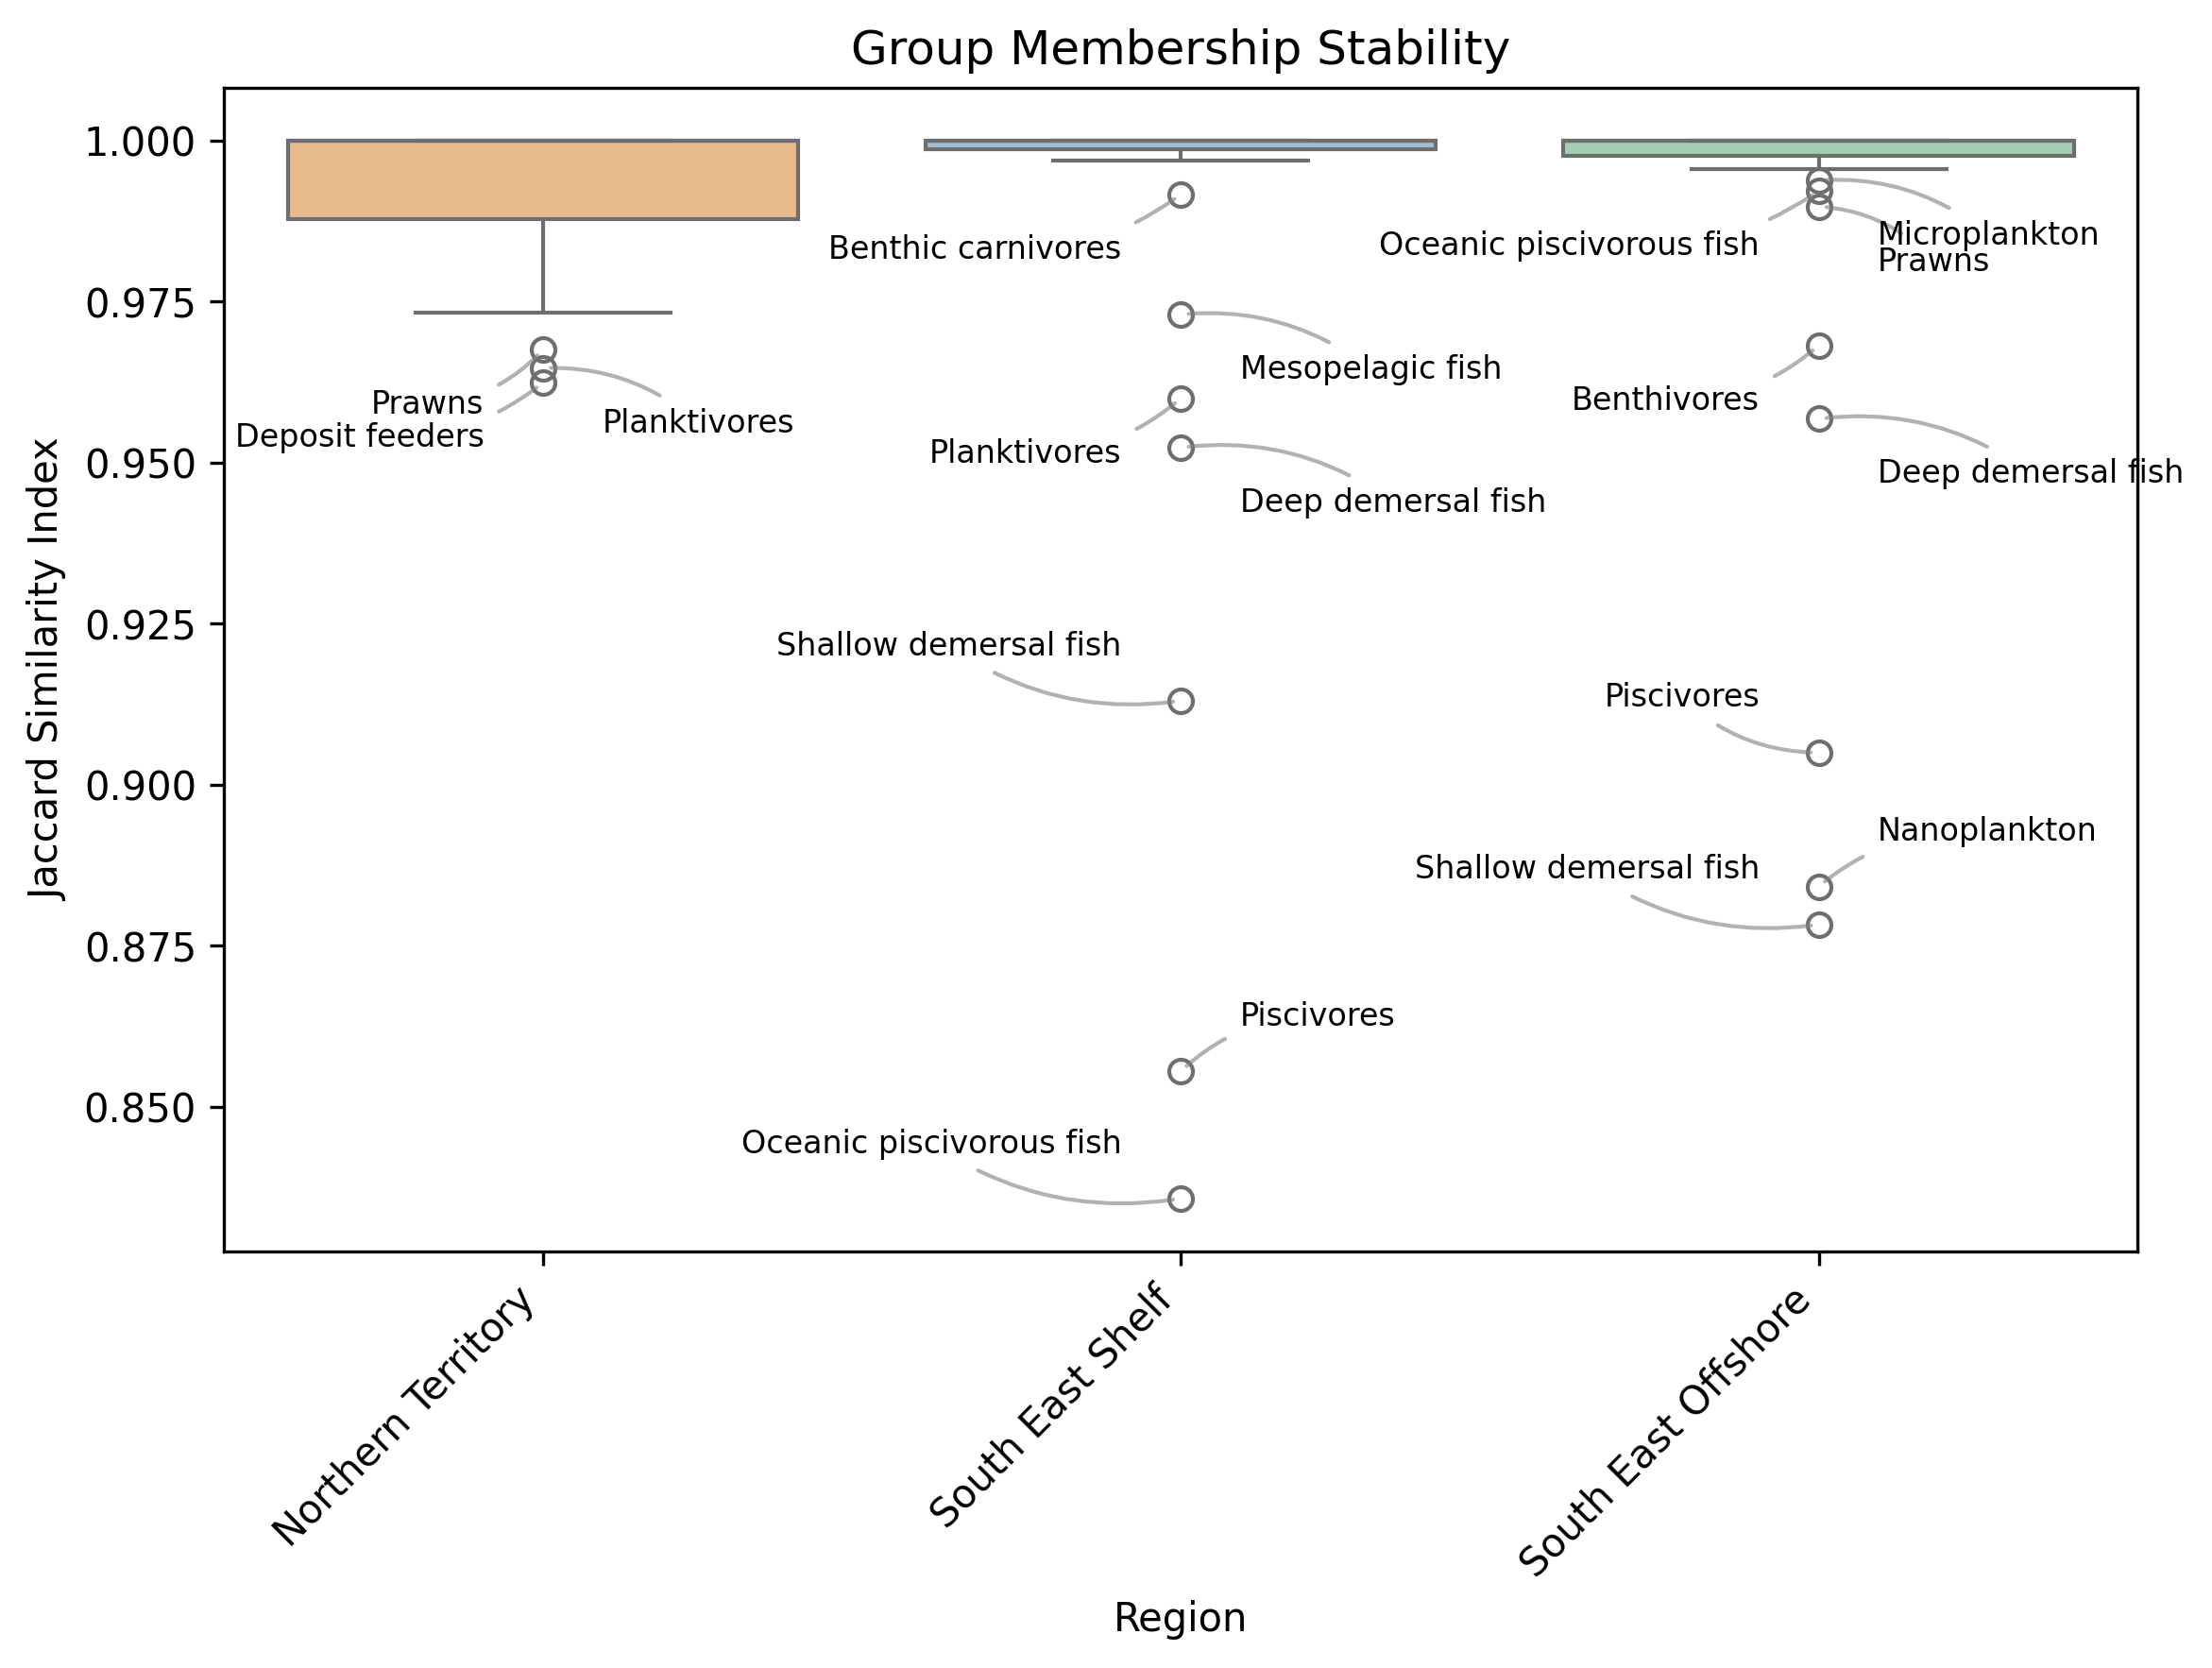
\includegraphics[width=\textwidth]{figures/regional_group_analysis.png}
    \caption{Group membership stability across three regions measured by Jaccard similarity index (0.85-1.0). Most groups show high stability (>0.95), with labelled points out-of-distribution outliers that exhibit lower stability.}
    \label{fig:regional_analysis}
\end{figure}

\begin{table}[htbp]
\centering
\caption{Dominant patterns of species classification instability across three study regions. The table presents the most frequent oscillation patterns between functional groups for species that were inconsistently classified across the five framework iterations. For each region, the total number of variably classified species is shown (representing less than 1.1\% of all species), along with the percentage distribution of different oscillation patterns.}
\label{tab:unstable_species}
\small
\begin{tabular}{llcc}
\hline
Region & Most Common Pattern & Count & \% of Total \\
\hline
Northern & Macrozoobenthos $\leftrightarrow$ Benthic infaunal carnivores & 28 & 27.2\% \\
Territory & Benthic filter feeders $\leftrightarrow$ Deposit feeders & 25 & 24.3\% \\
(103 species) & Prawns $\leftrightarrow$ Macrozoobenthos & 21 & 20.4\% \\
& Other patterns & 29 & 28.1\% \\
\hline
South East & Piscivores $\leftrightarrow$ Deep demersal fish & 42 & 33.6\% \\
Inshore & Benthic grazers $\leftrightarrow$ Benthic carnivores & 31 & 24.8\% \\
(125 species) & Planktivores $\leftrightarrow$ Mesopelagic fish & 28 & 22.4\% \\
& Other patterns & 24 & 19.2\% \\
\hline
South East & Benthic filter feeders $\leftrightarrow$ Benthic carnivores & 25 & 28.7\% \\
Offshore & Macrozoobenthos $\leftrightarrow$ Deep demersal fish & 22 & 25.3\% \\
(87 species) & Mesozooplankton $\leftrightarrow$ Macrozoobenthos & 18 & 20.7\% \\
& Other patterns & 22 & 25.3\% \\
\hline
\multicolumn{4}{p{0.95\textwidth}}{\small \textit{Note:} Arrows indicate group assignment oscillation between iterations. Complete species-level data available in Section S3 of the supplementary material.} \\
\hline
\end{tabular}
\end{table}


\subsection{Diet Matrix Reproducibility}
% Addressing Objective 2b: Assess consistency of diet matrix values

\subsubsection{Trophic Interaction Consistency}
The framework identified consistent trophic relationships across all regions, with the Northern Australia showing 358 interactions (58.7\% having stability scores > 0.7), South East shelf 380 interactions (51.3\% of which were stable), and South East Offshore 477 interactions (56.0\% stable). As shown in Figure \ref{fig:stability_distribution}, the distribution of stability scores across regions demonstrates that most interactions cluster above the 0.7 threshold, with a substantial proportion achieving near-perfect stability (scores approaching 1.0). Spearman correlations between iterations demonstrated that the relative proportions of different prey in predator diets remained fairly consistent across all regions (Northern Australia: $\rho = 0.72-0.89$; South East shelf: $\rho = 0.68-0.85$; South East Offshore: $\rho = 0.70-0.87$), even when absolute proportions varied. Detailed diet matrices for each region are provided in \ref{supp:diet_matrix}.

\begin{figure}[htbp]
    \centering
    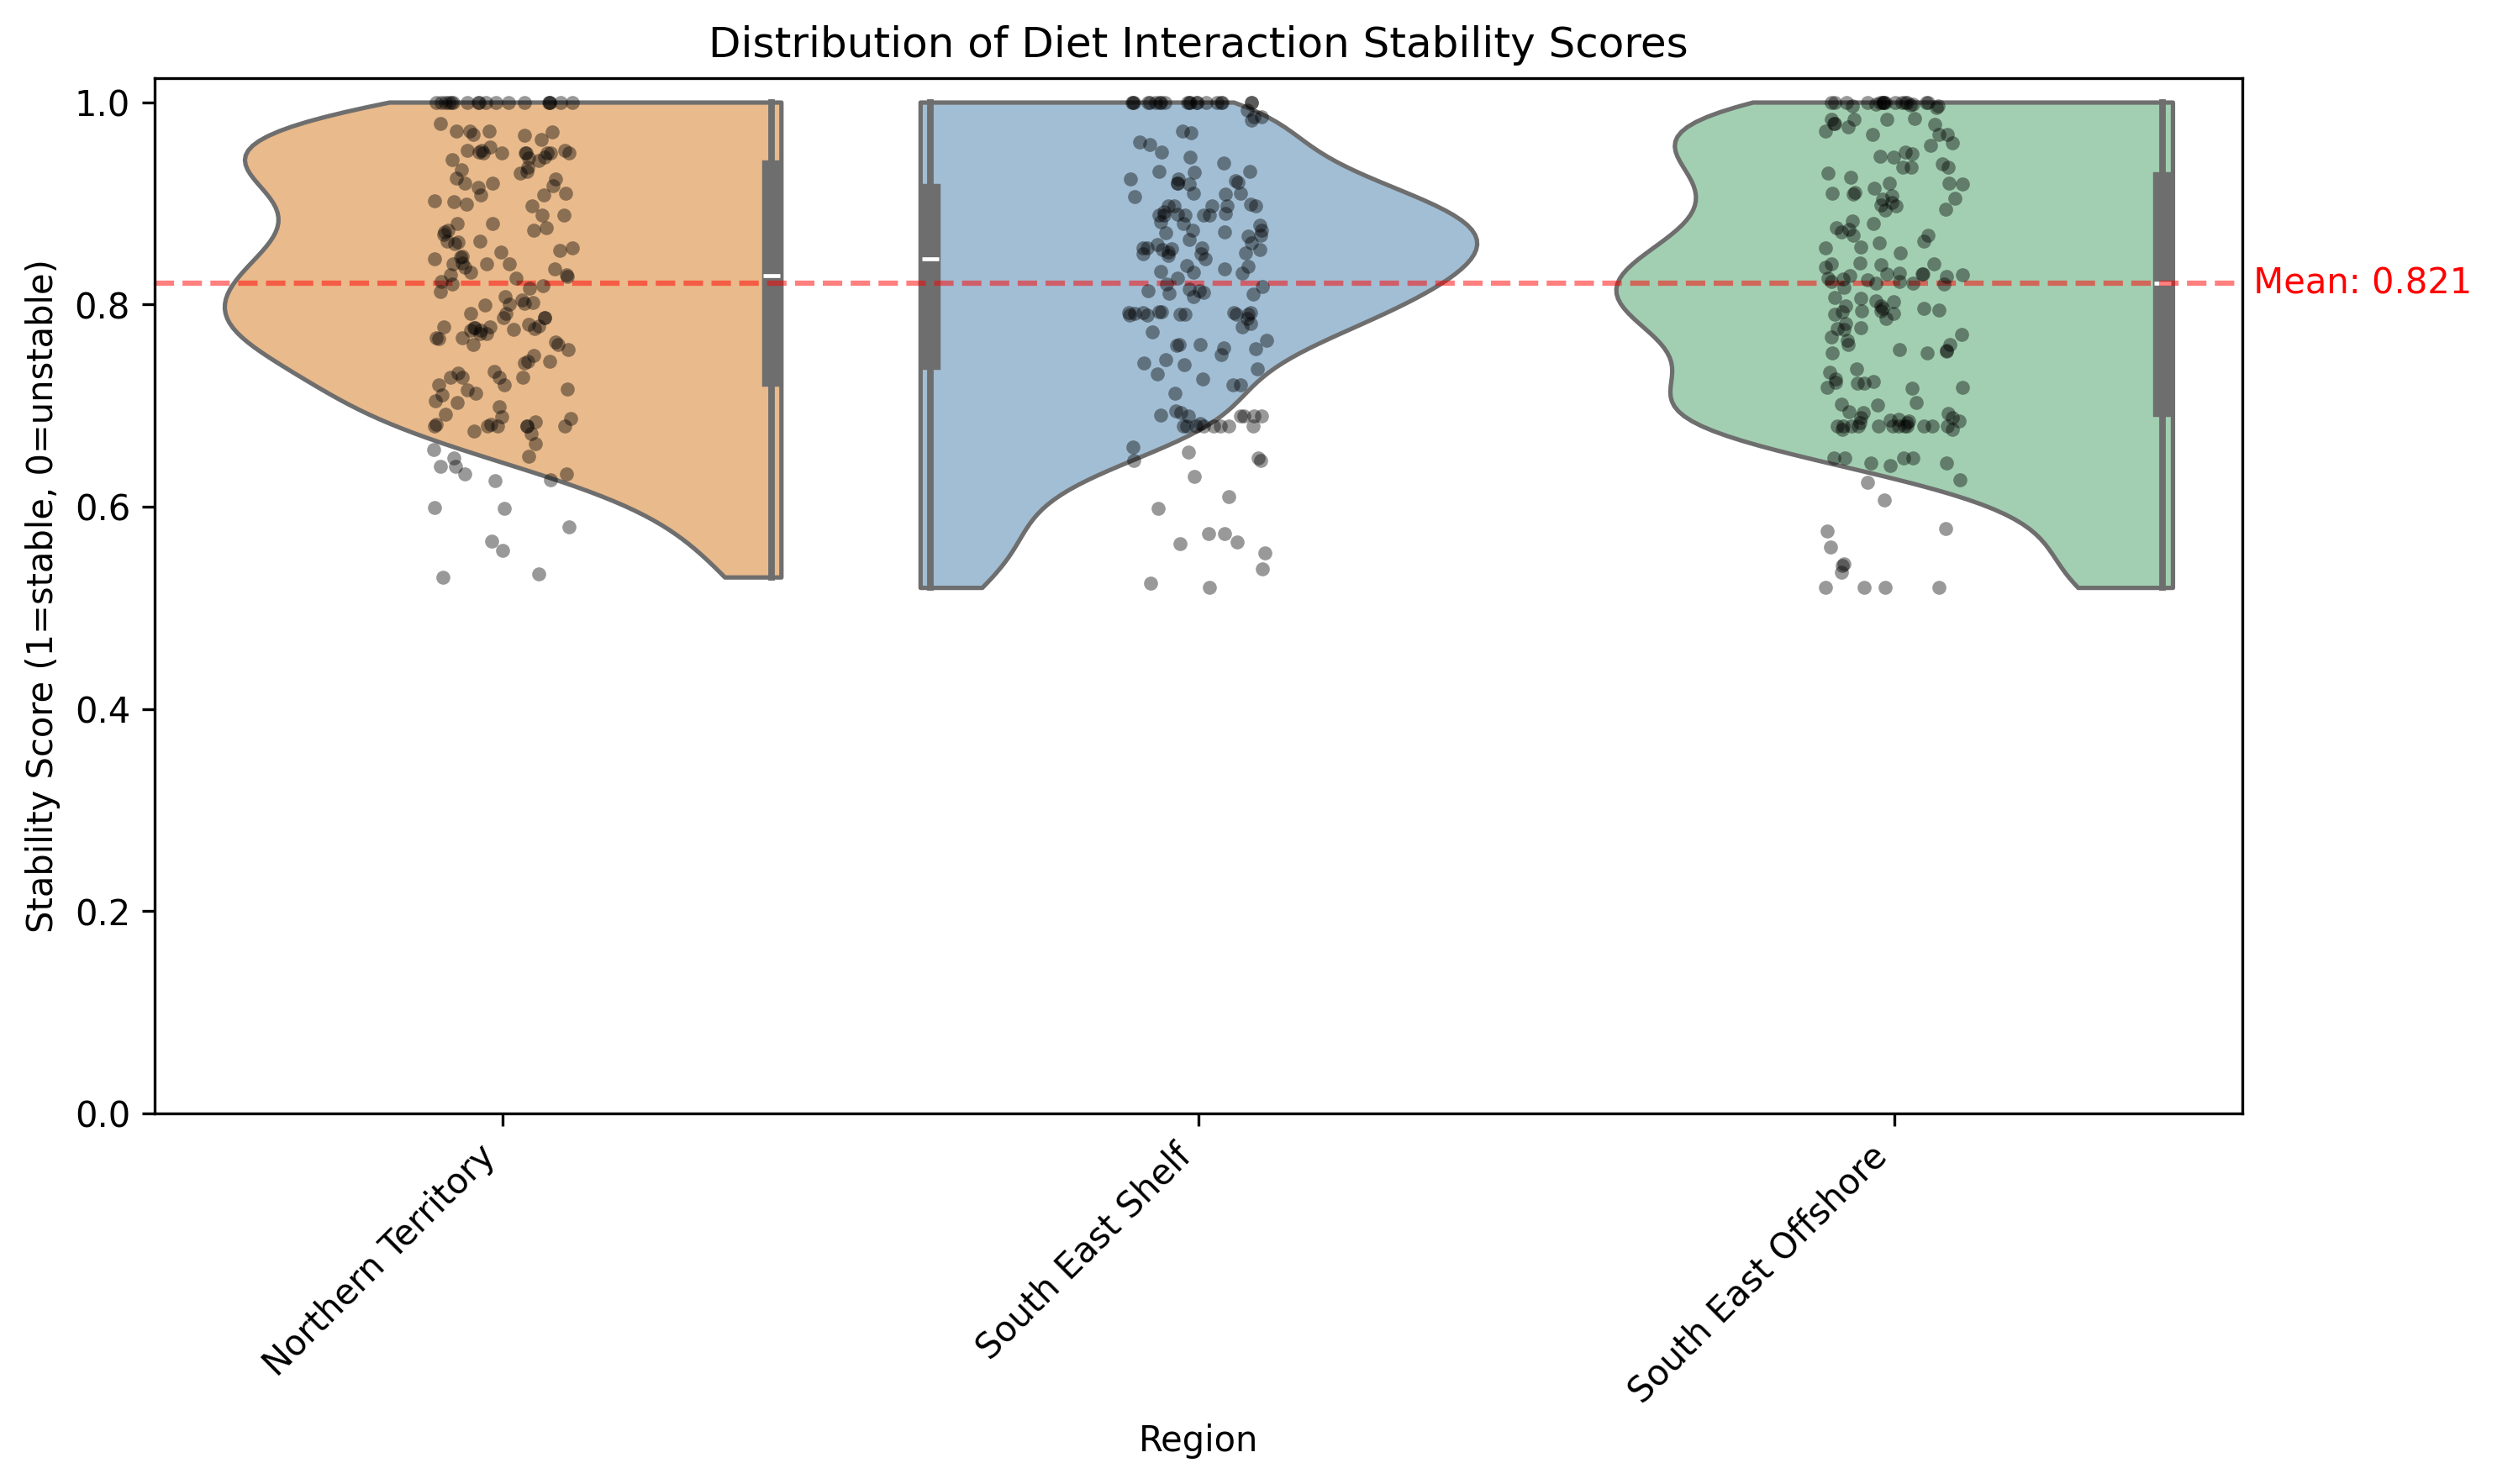
\includegraphics[width=\textwidth]{figures/stability_score_distribution.png}
    \caption{Distribution of diet interaction stability scores across regions for substantial interactions (those comprising more than 5\% of a predator's diet). Half-violin plots show the density of stability scores (1=stable, 0=unstable), with embedded box plots indicating quartiles and median. Individual points represent specific predator-prey interactions, and the red dashed line shows the mean stability score across all regions. The distributions are bounded at one, reflecting perfect stability, with most interactions showing scores above 0.7. Stability scores quantify the consistency of predator-prey interactions across iterations, where a score of 1.0 indicates the interaction was identified with identical diet proportions in all iterations, while lower scores reflect either variable diet proportions or inconsistent identification of the interaction. }
    \label{fig:stability_distribution}
\end{figure}

\subsection{Grouping and Diet Proportion Accuracy Assessment: Great Australian Bight Case Study}
% Addressing Objective 2c: Assess accuracy against expert-created matrices

\subsubsection{Taxonomic Grouping Accuracy}
To evaluate the ecological validity of AI-assigned functional groups, we conducted a detailed manual validation of 675 taxonomic grouping decisions. The results revealed that 75.3\% (508) of the AI's taxonomic assignments were fully correct, aligning with known ecological characteristics of the taxa. Additionally, 17.3\% (117) of assignments were partially correct, where the taxon fit some but not all aspects of the functional group description. For example, these included cases where the AI system designated a taxonomic group as 'deep' or 'slope' when they might inhabit both, or might designate a taxonomic group as 'large' or 'small' when members could be one or the other. Only 3.4\% (23) of assignments were clearly incorrect (demonstrable incorrect feeding strategy habitats), and 4.0\% (27) could not be definitively assessed due to limited ecological information about the taxa (mostly poorly researched deep-water taxonomies).

The accuracy of assignments varied considerably across functional groups (Figure \ref{fig:annotations_by_functional_group}). Many functional groups showed perfect or near-perfect assignment accuracy, including all assignments for albatross, pelagic sharks, small phytoplankton, mesozooplankton, small petrels, and several other well-defined groups. These groups typically have clear ecological niches and distinctive characteristics that facilitate accurate classification.

Functional groups with lower accuracy rates appeared to be constrained by limitations in the AI system's grouping template, particularly for specialized ecological niches. For example, waterfowl were frequently misclassified into the "Shags and cormorants" group, achieving only 33.3\% correct assignments with 50\% incorrect assignments. These errors revealed confusion between taxonomically related but ecologically distinct bird groups. Similarly, "Deep filter feeders" showed only 28.6\% correct assignments with 71.4\% partial assignments, highlighting challenges in classifying deep-sea organisms with complex or variable feeding strategies.

The analysis of partial assignments revealed several recurring patterns. Taxa associated with deep-sea environments (17 taxa) were frequently misclassified, likely due to limited ecological information and the complex nature of deep-sea ecosystems. Parasitic organisms (7 taxa) were also challenging to classify correctly, as they often have complex life cycles that span multiple functional roles. Filter feeders, detritivores, and grazers showed similar patterns of partial classification, typically due to their variable feeding strategies that may change based on environmental conditions or life stage.

\subsubsection{Diet Matrix Accuracy}
To evaluate the framework's accuracy against expert knowledge, we compared its output to an expert-derived Ecopath model of the Great Australian Bight ecosystem \citep{Fulton2018}. The framework demonstrated varying performance across functional groups, successfully matching 59 of 76 expert-defined groups (77.6\%). The framework omitted 17 groups present in the expert matrix, including several commercially important species (Southern Bluefin Tuna, Snapper, King George whiting, and Abalone) as well as Nanozooplankton. Conversely, it generated only two groups not present in the expert matrix (Offshore pelagic invertivores large and Slope large demersal omnivores).

As shown in Figure \ref{fig:gab_comparison}a, the framework demonstrated varying levels of agreement across different functional groups in identifying trophic interactions. The analysis revealed that 8.5\% of interactions were present in both matrices (dark purple), while 73.1\% were correctly identified as absent in both (light grey). The framework uniquely identified 14.5\% of interactions (teal) that were not present in the expert matrix, while missing 3.9\% of expert-identified interactions (yellow). Overall, the framework achieved an agreement rate of 81.6\% with the expert matrix, with a true positive rate (sensitivity) of 0.687 and a true negative rate (specificity) of 0.834.

The framework showed moderate success in capturing the quantitative aspects of diet proportions, with a Kappa coefficient of 0.38 with expert-assigned diet proportions. The distribution of absolute differences in diet proportions (Figure \ref{fig:gab_comparison}b) revealed that the majority of differences were relatively small, with approximately 80\% of the differences being less than 0.2. Detailed analysis showed a mean absolute difference of 0.110 (median: 0.058) in diet proportions for interactions present in both matrices. However, a long tail in the distribution (maximum difference: 0.865) indicates some cases where AI-generated proportions diverged substantially from expert values. This suggests that when the framework correctly identified a trophic interaction, it often estimated diet proportions within reasonable bounds of expert values, though with notable variations across different predator-prey combinations.

Further examination of the omitted groups revealed a pattern where the framework tended to miss specialized ecological groups, particularly those comprised of only a single species (e.g., Southern Bluefin Tuna, Snapper, King George whiting). This suggests a bias toward generalized classifications that may overlook management-relevant distinctions. This limitation was most evident in commercially important species that typically receive individual attention in expert-created models but were subsumed into broader functional groups by the framework. A comprehensive visualization of these differences across all functional groups is provided in \ref{supp:diet_matrix}.

\begin{figure}[htbp]
    \centering
    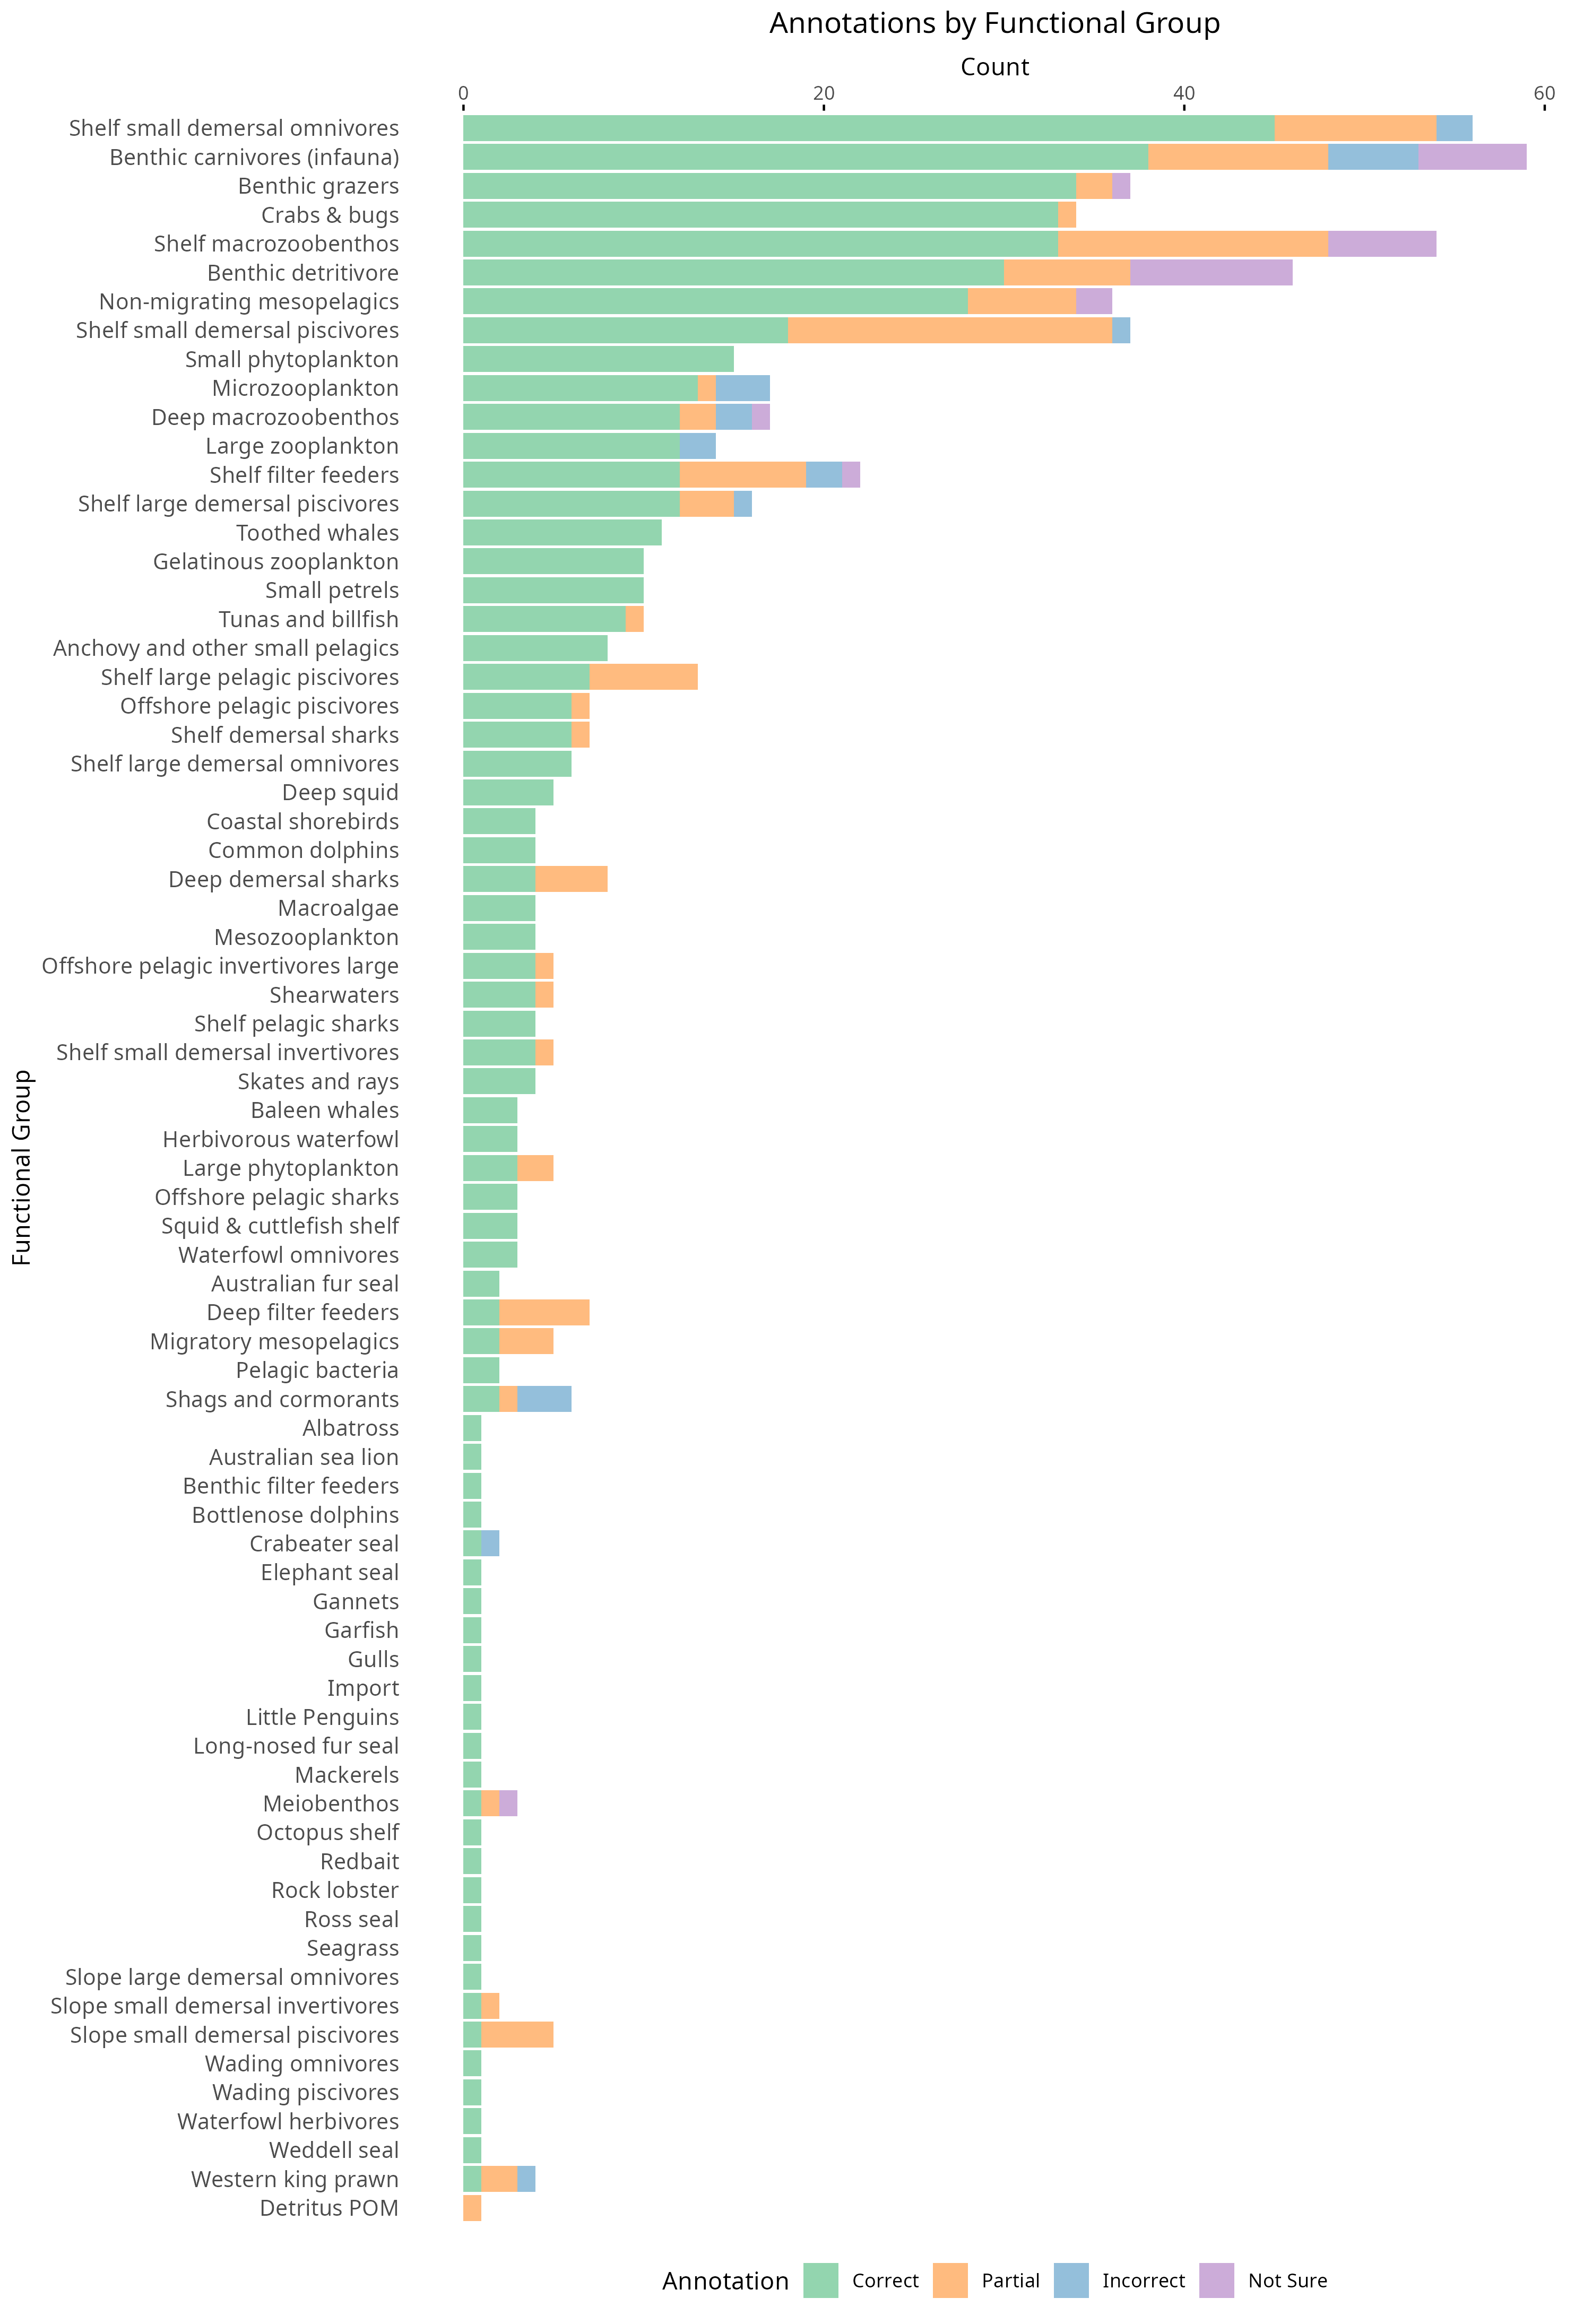
\includegraphics[width=\textwidth]{results/group_accuracy/results/annotations_by_functional_group.png}
    \caption{Accuracy of AI-assigned taxonomic groupings by functional group. The chart shows the percentage of correct (green), partial (orange), incorrect (blue), and uncertain (purple) assignments for each functional group.}
    \label{fig:annotations_by_functional_group}
\end{figure}

\begin{landscape}
\begin{figure}[htbp]
    \centering
    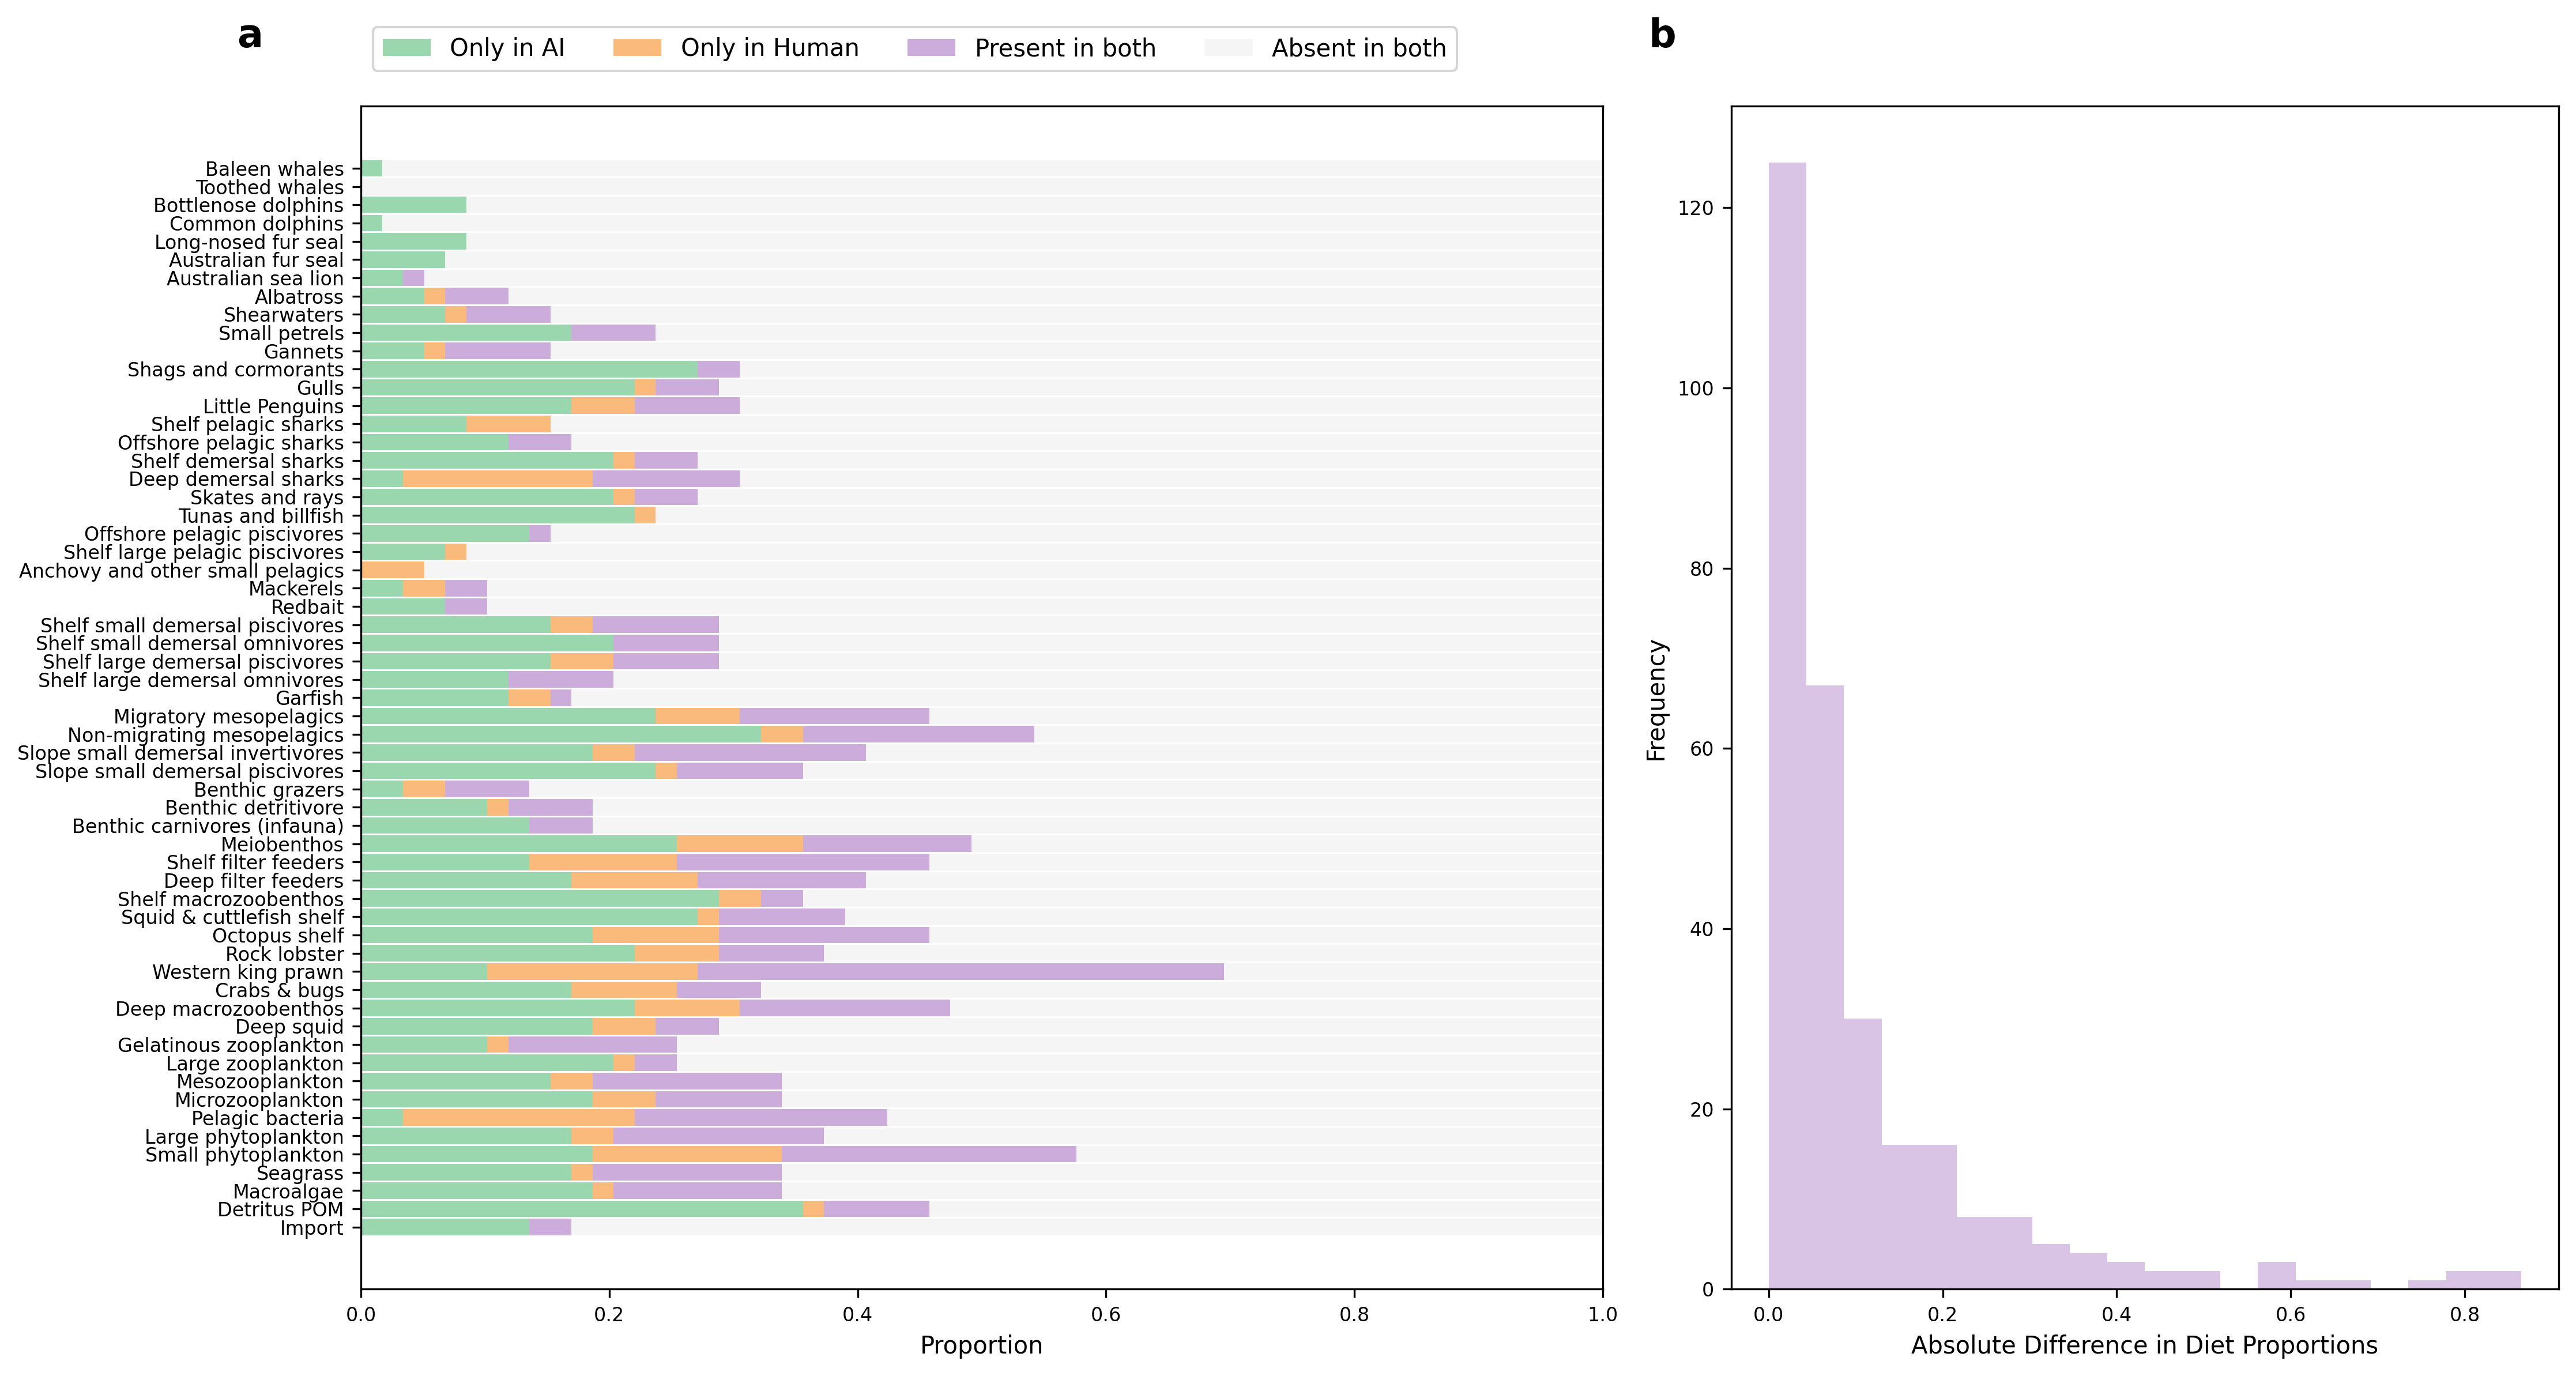
\includegraphics[width=1.2\paperwidth]{figures/diet_matrix_validation/simplified_comparison.png}
    \caption{Comparison of expert-created and AI-generated diet matrices for the Great Australian Bight ecosystem. (a) Presence-absence patterns showing the proportion of different interaction types across functional groups. Dark purple indicates interactions present in both matrices, orange shows expert-only interactions, teal shows AI-only interactions, and light grey indicates absence in both. (b) Distribution of absolute differences in diet proportions where both matrices indicate an interaction, showing the frequency of different magnitudes of disagreement between AI and expert estimates.}
    \label{fig:gab_comparison}
\end{figure}
\end{landscape}

\subsection{Framework Implementation and Performance}
% Addressing Objective 1: Present a systematic, AI-assisted framework for assembling and parameterizing EwE diet matrices

\subsubsection{Scale and Processing Efficiency}
We evaluated our framework through five independent runs across three distinct Australian regions, processing a total of 39,722 species. The framework handled 10,621 species in the Northern Australia's tropical reef ecosystem, 17,068 in the South East shelf's coastal and pelagic environments, and 12,033 in the South East Offshore's deep-water systems. 

\subsubsection{Computational Efficiency}
The computational requirements of the AI framework varied across regions. Total processing time ranged from 2.8 to 4.8 hours across regions. The most time-intensive stage was the downloading of biological data from online databases, accounting for approximately 70\% of the total processing time. Species identification typically required 0.01 hours, while the AI-driven species grouping process averaged 0.26 hours. Diet data collection and matrix construction required 0.7 and 0.04 hours respectively, with final parameter estimation taking 0.20 hours. On average, the framework required 0.7 seconds per species for data downloading and 0.2 seconds per species for diet data collection, though these rates varied considerably between regions due to differences in data availability and species complexity.
\begin{table}[htbp]
\centering
\footnotesize
\caption{Computational requirements by region and processing stage}
\label{tab:timing_analysis}
\begin{tabular}{lccccccc}
\hline
Region & Species & \multicolumn{6}{c}{Processing Time (hours)} \\
\cline{3-8}
 & Count & Identification & Data & Grouping & Diet & Matrix & Parameter \\
 & & & Download & & Collection & Construction & Estimation \\
\hline
v2 NorthernTerritory & 11,362 & 0.01 & 2.2 & 0.2 & 0.2 & 0.04 & 0.2 \\
v2 SouthEastInshore & 13,901 & 0.01 & 2.8 & 0.2 & 1.6 & 0.04 & 0.2 \\
v2 SouthEastOffshore & 15,821 & 0.01 & 3.3 & 0.4 & 0.3 & 0.04 & --- \\
\hline
\end{tabular}
\vspace{1ex}
\end{table}


